\documentclass[11pt]{article}
\usepackage[cm]{fullpage}

\usepackage{tikz}
\usepackage{amsmath}

\usepackage{listings}
\lstset{basicstyle=\ttfamily\small}
\lstset{literate={~} {$\sim$}{1}}
\lstset{showstringspaces=false}
\lstset{language=Python}

\newcommand{\linp}[1]{\lstinputlisting{#1}{}}
\newcommand{\linl}[1]{\lstinline{#1}{}}

\usepackage[cm]{fullpage}
\usepackage{mathtools} %includes amsmath
\usepackage{lmodern}
\usepackage{scrextend}
\usepackage{enumitem}
\usepackage{hyperref}
\usepackage{tikz}
\newcommand{\ttf}[1]{{\ttfamily #1}}
\newcommand{\bo}[1]{\ensuremath{\mathbf{#1}}}
\newcommand{\s}{\textbackslash}
\renewcommand{\sp}{\ \ \ \ \ \ \ \ \ \ }
\newcommand{\pt}{\partial}
\newcommand{\fr}[2]{\dfrac{#1}{#2}}
\newcommand{\pr}[1]{\left(#1\right)}
\newcommand{\ord}[1]{\ensuremath{^{(#1)}}}
\newcommand{\ma}[1]{\left(\begin{matrix}#1\end{matrix}\right)}
\newcommand{\pd}[3]{\ensuremath{ \dfrac{ \partial^{#1} #2 }{\partial #3 ^{#1}}}}
\newcommand{\bigo}{\ensuremath{\mathcal{O}}}
\newcommand{\eth}{\ensuremath{^\text{th}}}
\newcommand{\ld}{\ensuremath{\ldots}}
\newcommand{\miniar}[1]{\ensuremath{\begin{smallmatrix}#1\end{smallmatrix}}}

\title{Programming Project 2 Theory\\
\textit{Central Difference 2$^\text{nd}$ Derivative Formulas}}
\date{}
\author{}

\begin{document}
\maketitle
\vspace{-1cm}

\noindent
If you have taken a Calculus I, you are probably already familiar with
one finite difference formula:
\begin{align*}
    f'(x) = \lim_{h\rightarrow0} \fr{f(x+h)-f(x)}{h}
\end{align*}
In applied mathematics this is called a
forward-difference first-derivative, i.e.~a first derivative determined by
displacing the function argument by $+h$. An example of a central-difference
first-derivative formula is
\begin{align*}
    f'(x) = \lim_{h\rightarrow0} \fr{f(x+h)-f(x-h)}{2h} 
\end{align*}
which involves both forward and backward displacements.

A straightforward method of deriving these formulas starts from a
Taylor expansion.
\begin{align}
    f(x) 
    =&\
    \sum_{n=0}^\infty \fr{1}{n!}
    \left.\pd{n}{f}{x}\right|_{x=0} x^n
\end{align}
Which, for our purposes, is more conveniently expressed as
\begin{align}
    f(x) =&\
      f_0 + f_0\ord{1}x + \fr{1}{2!}f_0\ord{2}x^2
      + \fr{1}{3!}f_0\ord{3}x^3 + \bigo(x^4)
\end{align}
where $f_0\ord{n}$ denotes the value of the $n\eth$ derivative of $f$ at $x=0$.
The last term, $\bigo(x^4)$, describes the magnitude of the error incurred by
truncating the Taylor expansion at a particular point.

The basic strategy used to derive expressions for the derivatives is to plug in a grid of $x$-values $\{x_k\}$, yielding a series of equations, and then solve
for the derivatives in terms of the function values at these points
$\{f(x_k)\}$. Here we will take the ``uniform grid'' approach, in which we use
$x$ values with a fixed interval $h$ between them
$\{\ld,-2h,-h,0,+h,+2h,\ld\}$.

\subsection*{Derivatives of one variable}
To get a first approximation of the first and second derivatives in one
variable, we only need three points from our grid $\{-h,0,+h\}$.
Let $f_{\pm k}$ represent $f(\pm kh)$ to keep things a little bit neater.
\begin{align*}
    f_{+1} =&\
    f_0 + f\ord{1}_0 h + \fr{1}{2!}f\ord{2}_0 h^2
    +\bigo(h^3)\\
    f_{-1} =&\
    f_0 - f\ord{1}_0 h + \fr{1}{2!}f\ord{2}_0 h^2
    -\bigo(h^3)
\end{align*}
When we subtract the two equations, the even powers
of $h$ cancel and we can solve for the first derivative.
\begin{align*}
    f\ord{1}_0 =&\ \fr{f_{+1}-f_{-1}}{2h} +\bigo(h^2)
&&\iff
&&
    \pr{\fr{\pt f}{\pt x}}_{x=x_0} = 
    \fr{f(x_0+h)-f(x_0-h)}{2h}+\bigo(h^2)
\\
\intertext{Adding the two equations cancels even powers, allowing us to solve for the
second derivative.}
    f\ord{2}_0 =&\ \fr{f_{+1}+f_{-1}-2f_0}{h^2} +\bigo(h^2)
&&\iff
&&
    \pr{\fr{\pt^2f}{\pt x^2}}_{x=x_0} = 
    \fr{f(x_0+h)+f(x_0-h)-2f(x_0)}{h^2}+\bigo(h^2)
\end{align*}

\subsection*{Mixed partials}
The Taylor expansion
for a multivariate function is
\begin{align*}
    f(x_1,\ld,x_n) =&\ 
    f_0
    +\sum_{i=1}^n
    \pr{\fr{\pt f}{\pt x_i}}_0x_i
    +\fr{1}{2!}\sum_{i,j=1}^n
    \pr{\fr{\pt^2f}{\pt x_i\pt x_j}}_0x_ix_j
    +\fr{1}{3!}\sum_{i,j,k=1}^n
    \pr{\fr{\pt^3f}{\pt x_i\pt x_j\pt x_k}}_0
    x_ix_jx_k
    +\ld
\end{align*}
In order to determine the elements of $f$'s second-derivative (Hessian) matrix $H_{ij}=\fr{\pt^2 f}{\pt x_i\pt x_j}$ we need mixed
partial derivatives of the form $\fr{\pt^2f}{\pt x\pt y}$
in addition to the one-variable formulas above, which give us the diagonal elements.
These can be derived from a bivariate Taylor expansion.
\begin{align*}
    f(x,y) =&\
    f_{0,0} + f_{0,0}\ord{1,0}x + f_{0,0}\ord{0,1}y
    +\fr{1}{2!} f_{0,0}\ord{2,0}x^2
    +f_{0,0}\ord{1,1}xy
    +\fr{1}{2!} f_{0,0}\ord{0,2}y^2
    +\ld
\\\intertext{The equations for double-forward and double-backward displacement are then}
    f_{+1,+1} =&\ 
    f_{0,0} + f\ord{1,0}_{0,0}h+f\ord{0,1}_{0,0}h + 
    \fr{1}{2!}f\ord{2,0}_{0,0}h^2+f\ord{1,1}_{0,0} h^2
    +\fr{1}{2!} f\ord{0,2}_{0,0}h^2
    +\bigo(h^3)
    \\
    f_{-1,-1} =&\ 
    f_{0,0} - f\ord{1,0}_{0,0}h-f\ord{0,1}_{0,0}h + 
    \fr{1}{2!}f\ord{2,0}_{0,0}h^2+f\ord{1,1}_{0,0} h^2
    +\fr{1}{2!} f\ord{0,2}_{0,0}h^2
    -\bigo(h^3)\ .
\end{align*}
Adding these equations and rearranging, we obtain
\begin{align*}
    f\ord{1,1}_{0,0} =&\ 
    \fr{f_{+1,+1}+f_{-1,-1}-2f_{0,0} }{2h^2}
    -\fr{f\ord{2,0}_{0,0} + f\ord{0,2}_{0,0}}{2}
    +\bigo(h^2)\ .
\end{align*}
Since $f\ord{2,0}_{0,0}, f\ord{0,2}_{0,0}$ are partials with
respect to a single variable, we can plug in the expressions
derived above
\begin{align*}
    f\ord{1,1}_{0,0} =&\ 
    \fr{f_{+1,+1}+f_{-1,-1}
        -f_{+1,0}-f_{-1,0}
        -f_{0,+1}-f_{0,-1}+2f_{0,0}
    }{2h^2}
    +\bigo(h^2)
\end{align*}
giving the following central-difference formula for mixed second derivatives.
{\small
\begin{align*}
    &\pr{\fr{\pt^2f}{\pt x\pt y}}_{\miniar{x=x_0\\y=y_0}}\\ & \ \ =
    \fr{f(x_0+h,y_0+h)+f(x_0-h,y_0-h)-f(x_0+h,y_0)-f(x_0-h,y_0)-f(x_0,y_0+h)-f(x_0,y_0-h)+2f(x_0,y_0)}{2h^2} \\ &\sp + \bigo(h^2)
\end{align*}}
These expressions are sometimes described by to the grid of points used
in them. In this case, the grid is
\begin{center}
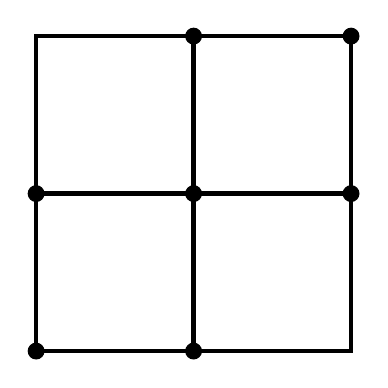
\begin{tikzpicture}[scale=2]
\draw [ultra thick] (-1,-1)--(-1,+1)--(+1,+1)--(+1,-1)--(-1,-1);
\draw [ultra thick] (0,-1)--(0,+1);
\draw [ultra thick] (-1,0)--(+1,0);
\draw[fill] (+1,+1) circle [radius=0.05];
\draw[fill] (+1,0) circle [radius=0.05];
\draw[fill] (0,+1) circle [radius=0.05];
\draw[fill] (0,0) circle [radius=0.05];
\draw[fill] (-1,-1) circle [radius=0.05];
\draw[fill] (-1,0) circle [radius=0.05];
\draw[fill] (0,-1) circle [radius=0.05];
\end{tikzpicture}
\end{center}
where the middle point is the origin and all line segments have length $h$.

\end{document}
